%% This is an example first chapter.  You should put chapter/appendix that you
%% write into a separate file, and add a line \include{yourfilename} to
%% main.tex, where `yourfilename.tex' is the name of the chapter/appendix file.
%% You can process specific files by typing their names in at the 
%% \files=
%% prompt when you run the file main.tex through LaTeX.

\chapter{LGR Performance and Field Characterization} \label{ch3}

In this chapter the LGR electrical and magnetic are discussed and measured. All simulations were completed in ANSYS HFSS a full-wave electromagnetic simulation tool. 

\section{Quality Factor}\label{quality}

As mentioned in section \ref{resonant_enhc}, The quality (or Q) factor of an oscillator quantifies how often (in terms of the oscillation period) the energy will oscillate back and forth until its initial amplitude is reduced by a factor of $1/e$. At critical coupling ($\beta = 1$) the intrinsic Q ($Q_0$) of the resonator (which quantifies the oscillation lifetime due to resistive losses) is calculated as the inverse of its fractional bandwidth ($FBW$),
\begin{equation}
Q_0 = \frac{1}{FBW} = \frac{f_0}{\Delta_{3dB}}.
\end{equation} 
The fractional bandwidth however is calculated from the loaded Q ($Q_L$) which takes into account coupling losses due to power reflection at the exciter antenna/LGR interface. Incorporating these reflections is achieved by assigning an external Q ($Q_e$) to account for these losses. $Q_e$ then combines with $Q_0$ in a parallel configuration
\begin{equation}
\frac{1}{Q_L} = \frac{1}{Q_0} + \frac{1}{Q_e},
\end{equation} 
to yield $Q_L$. The intrinsic Q, $Q_0$, and the external Q, $Q_e$, characterise the most dominant loss mechanisms of the device. Other loss mechanisms and their contribution to $Q_L$ are discussed in reference \cite{piasecki1993field}; they include, but are not limited to, loss in a sample, radiation losses, surface wave losses, hand-shaking (if not properly shielded), etc..

Since the quality factor is inversely proportional to the resonator bandwidth the LGR needs to exhibit fairly low Q in order to address all eight NV resonances and their shifts due to an external field. The LGR was thus designed to accommodate an NV ensemble that has been split using an up-to 14 gauss biasing field $B_0$. Since the NV gyromagnetic ratio ($\gamma_B$) is 2.8 MHz/gauss, this corresponds to an ideal bandwidth of 78 MHz and, at 2.87 GHz, a Q of $\sim$ 36. In addition to a wide dynamic range, a low Q allows for the use of concatenated pulse sequences without employing additional methods to evacuate power from the resonator before the next pulse is applied (e.g. active cancellation). 

\subsection{Ringdown time}\label{ringdown}

As mentioned above, in order to apply concatenated MW pulses to a sample in the LGR (as is done often in NMR and NV applications \cite{wang2012comparison, carr1954effects}) the power oscillating in the cavity must be evacuated or dissipated in between pulses. One method used is to apply active cancellation techniques that either introduce extra components to the excitation circuitry to abruptly de-tune the resonator before the next pulse is applied  \cite{peshkovsky2005rf} or apply a secondary pulse that is designed to destructively interfere with the cavity ring-down \cite{Franck2015Active}. Another, and also the technique applied here, is to make the resonator intrinsically lossy and therefore dissipate the left-over power in the cavity as either heat or radiation. To calculate the ring-down time $\tau_{ring}$ of the LGR we apply a damping exponential to the field within the cavity such that $B(t) = B_{init}e^{-\pi f_0t/Q}$ (neglecting any phase caused by a shift in the resonant frequency), and solving for the time $t$ at which the amplitude has decreased to $1/e \cdot B_{init}$. Doing this yields
\begin{equation}\label{eqn33}
\tau_{ring} = \frac{Q}{\pi f_0}.
\end{equation} 
Using equation \ref{eqn33} and the bandwidth and center frequency extracted from the measured data in Figure \ref{LGR_tuning}, one calculates $\tau_{ring} = 4$ ns which is sufficient for standard NV and NMR pulsed protocols \cite{Smeltzer2009Robust,Jelezko2004Observation,Steiner2010Universal}.

\section{Simulating the Magnetic Field} \label{simField}

The $B_1$ field distribution in the center loop of the LGR was simulated using the full-wave electromagnetics simulation suite ANSYS HFSS. The simulation includes the 200 $\upmu$m dielectric shims and the full exciter circuit depicted in Figures \ref{LGR_Exciter} and \ref{LGR_drawing}. The solution type was set to "driven modal" since the exciter board has a single trace interconnect and thus requires the solution of TE and TM propagation modes. Figure \ref{LGR_simulated} shows the $B_1$ distribution computed by HFSS at an input power of 42 dBm. The exciter board (which extends over the LGR center loop along the line $x = y$ in the figure) clearly imparts a small perturbation on the otherwise radially symmetric field. The simulation predicts $B_1 \approx 4.8$ gauss at the LGR center and a maximum field of $B_1 \approx 5.4$ gauss at the perimeter. Two metrics are used to quantitatively characterize 2D regions of homogeneity, the fractional root-mean-square inhomogeneity $\sigma_{rms}$ calculated as 
\begin{equation}\label{sigma_rms}
\sigma_{rms} = \sqrt{\frac{\Sigma_{i = 1}^N|B_{1,i}|^2}{N}} \cdot \mu_N^{-1},
\end{equation}
where $i$ is an index over all $B_1$ field values in the region, $N$ is the total number of values, and $\mu_N$ is the mean of all $N$ values, and the fractional peak-to-peak variation $\sigma_{pp}$ calculated as
\begin{equation}\label{sigma_pp}
\sigma_{pp} = \frac{\left[B_1^{max} - B_1^{min}\right]}{\mu_N}.
\end{equation} 
The use of both metrics facilitates comparison with alternative existing designs. Within a 32 mm\textsuperscript{2} circular area centered in the LGR central loop, simulations indicate $\sigma_{rms} = 3.8\%$ and $\sigma_{pp} = 11\%$, whereas in a smaller 11 mm\textsuperscript{2} circular area, simulations indicate $\sigma_{rms} = 1\%$ and $\sigma_{pp} = 2\%$.

\begin{figure}[t!]
\centering
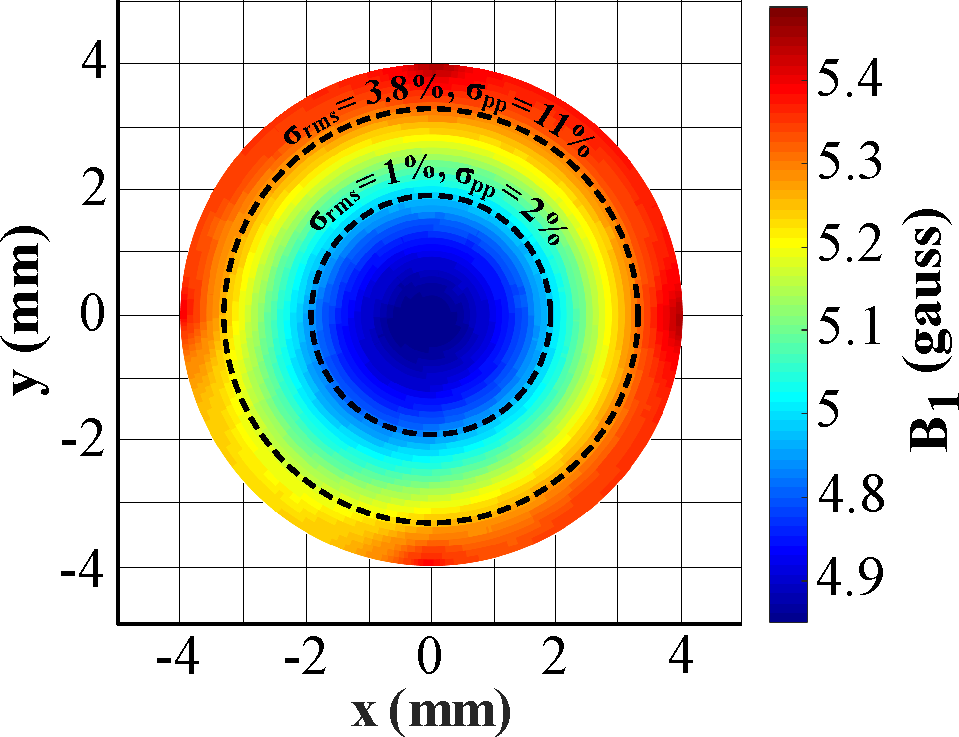
\includegraphics[scale = 0.75]{FieldSimulation.pdf}  
\caption{\textbf{Simulated magnetic field} Top-down cross section of center loop of LGR. Slice is taken at half height h. Simulations suggest the $B_1$ field distribution
should be approximately radially symmetric, with the leading order deviation resulting from the exciter antenna. Dashed lines indicate the 32 mm\textsuperscript{2} and 11mm\textsuperscript{2} areas within which the $B_1$ field uniformity is evaluated.}
\label{LGR_simulated}
\end{figure}

As a three dimensional cavity resonator, the LGR provides better axial field uniformity than planar-only geometries \cite{floch2016towards,kapitanova2017dielectric,angerer2016collective}. Figure \ref{LGR_axial_simulated} plots the simulated $B_1$ along the LGR's symmetry axis, illustrating the improved axial field uniformity possible with three-dimensional cavity
resonators, compared to that of planar-only geometries. The presence of the split ring resonator at $z = 4.024$ mm perturbs $B_1$ inside the LGR, shifting the point of maximal $B_1$ down by 0.4 mm, away from the split-ring resonator. Within a cylindrical volume of 3.14 mm\textsuperscript{3} (1 mm radius and 1 mm thickness), centered around the point of maximal $B_1$, the simulations predicts $\sigma_{rms} = 0.78\%$ and $\sigma_{pp} = 3.7\%$. For a larger cylindrical volume of 12.6 mm\textsuperscript{3} (2 mm radius and 1 mm thickness), the simulation predicts $\sigma_{rms} = 2\%$ and $\sigma_{pp} = 8\%$. These dimensions are comparable to those of commercially available single-crystal diamonds. Additionally, Figure \ref{LGR_axial_simulated} gives 1D regions of homogeneity along the LGR symmetry axis.

\begin{figure}[t!]
\centering
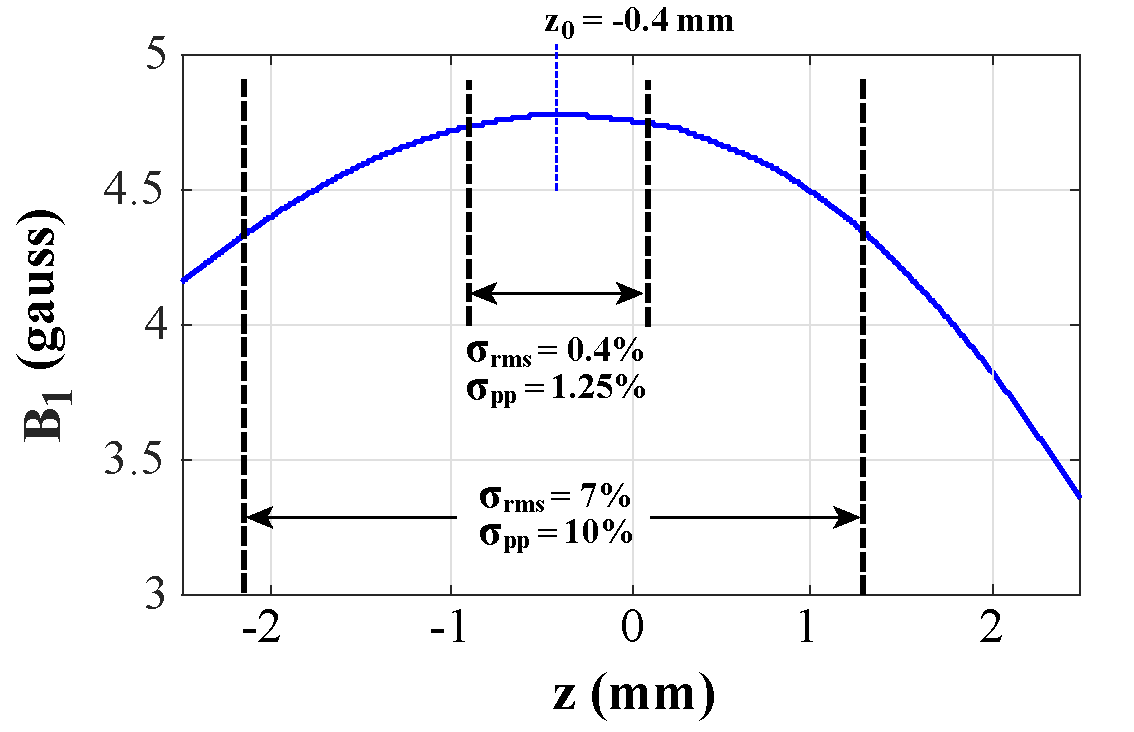
\includegraphics[scale = 0.7]{Figure_B_2.pdf}  
\caption{\textbf{Simulated $B_1$ field along LGR symmetry axis.} The symmetry plane of the LGR is located at $z = 0$ mm. The edges of the LGR are at $z = \pm 2.5$ mm, and the split-ring resonator is located at $z = 4.024$ mm. The presence of the split-ring resonator shifts the point of maximal $B_1$ off-center to $z_0 = -0.4$ mm.}
\label{LGR_axial_simulated}
\end{figure}

\section{Measuring the Magnetic Field} \label{field}

Measuring the magnetic field distribution within the central loop of the LGR can be done in several ways. The simplest is to raster scan a magnetic probe across the cross section to be measured. However there are many drawbacks to this method. First, the spatial resolution is set by the size of the probe tip. Figure \ref{LGR_probe} shows the normalized magnetic field distribution of the LGR, measured by a 100B Beehive magnetic probe. The shielded loop diameter of the probe is 1 mm and thus the resolution is poor. Second, the probe has very little access to the center of the cavity. The data in Figure \ref{LGR_probe} was, for example, taken 1 mm above the LGR center loop; a region in which the magnetic field is highly divergent. Since the magnetic loop only measures the component of the field that lies parallel with its cental axis this provides a limited picture of the total field distribution. Finally, the proximity of the probe to the LGR perturbs the field and thus the distribution measured is an altered version of the field in the unperturbed scenario. 

Another method--with similar drawbacks--is to measure the cavity transmission characteristics under intentional perturbation by a metal probe tip. By moving the perturbing probe tip, the transmission parameter $S_{21}$ (when an out-coupler loop is placed into one of the lateral loops) changes proportional to the field at the point of measurement. Thus, if the metal tip is scanned across the cavity, a picture of the field distribution can be extracted.  

Since the LGR in this thesis is designed to supply MWs to NV centers, one can utilize NV centers to, in turn, measure the strength of the supplied MWs. If the period of the Rabi frequency (as described in section \ref{Rabi}) can be determined, then one can, using a simple relation, calculate the magnitude of $B_1$ (section \ref{measurement} equation \ref{B1fromRabi}). This measurement of the field does not suffer from the drawbacks of the other two mentioned above and thus, it's the method employed in this thesis. The following subsections describe the measurement apparatus, measurement process, and calculations used to infer the strength of the $B_1$ field at various points within the LGR center loop.

\begin{figure}[t!]
\centering
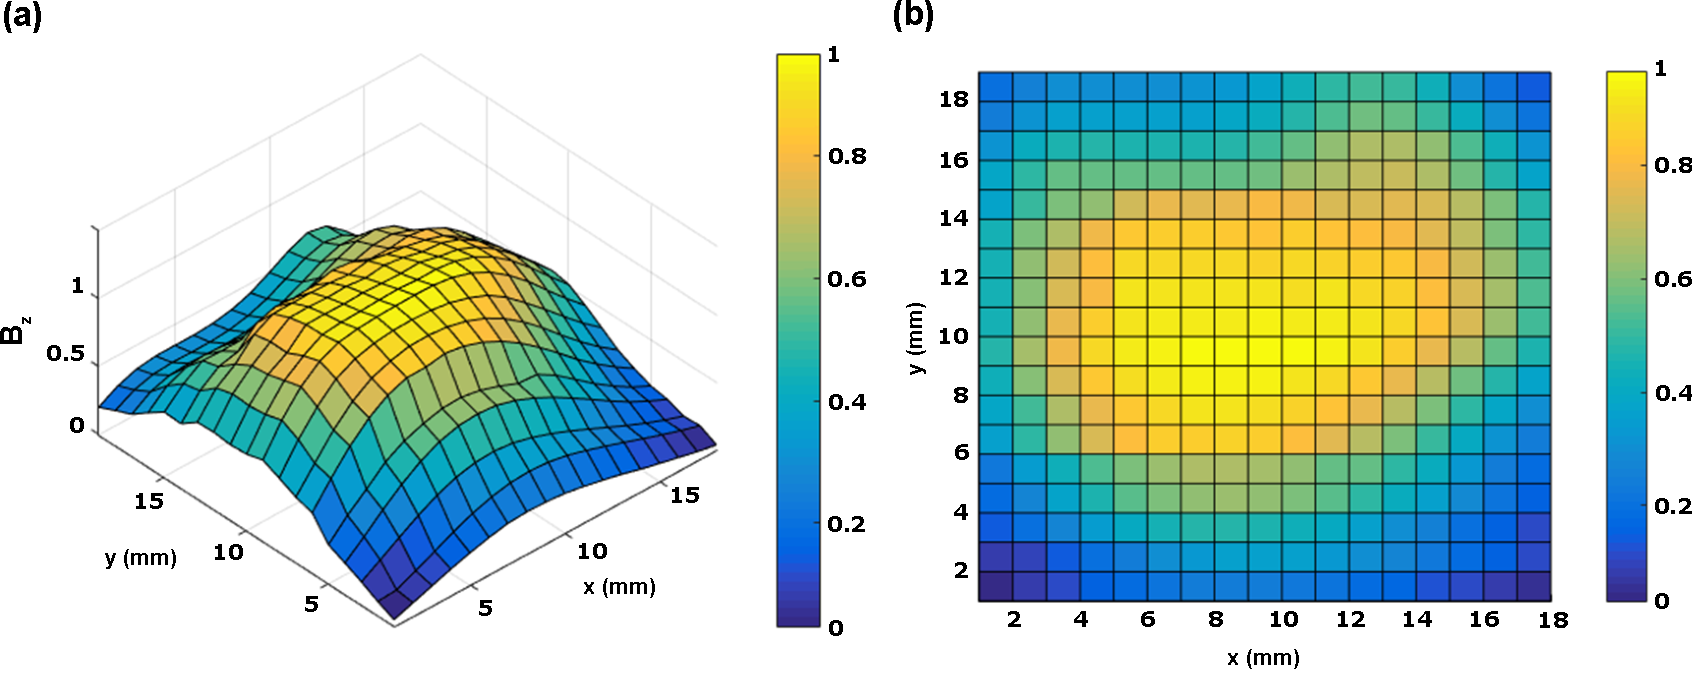
\includegraphics[width = \textwidth]{probefield.pdf}  
\caption{\textbf{$B_z$ component of field measured with probe} \textbf{a)} 3D surface plot of $B_z$ field distribution using a Beehive 100B magnetic field probe. Color bar units are normalized magnetic field. Normalized to their maximum value. \textbf{b)} Same data as in a) but top-down view. }
\label{LGR_probe}
\end{figure}

\begin{landscape}
\begin{figure}[b!]
\centering
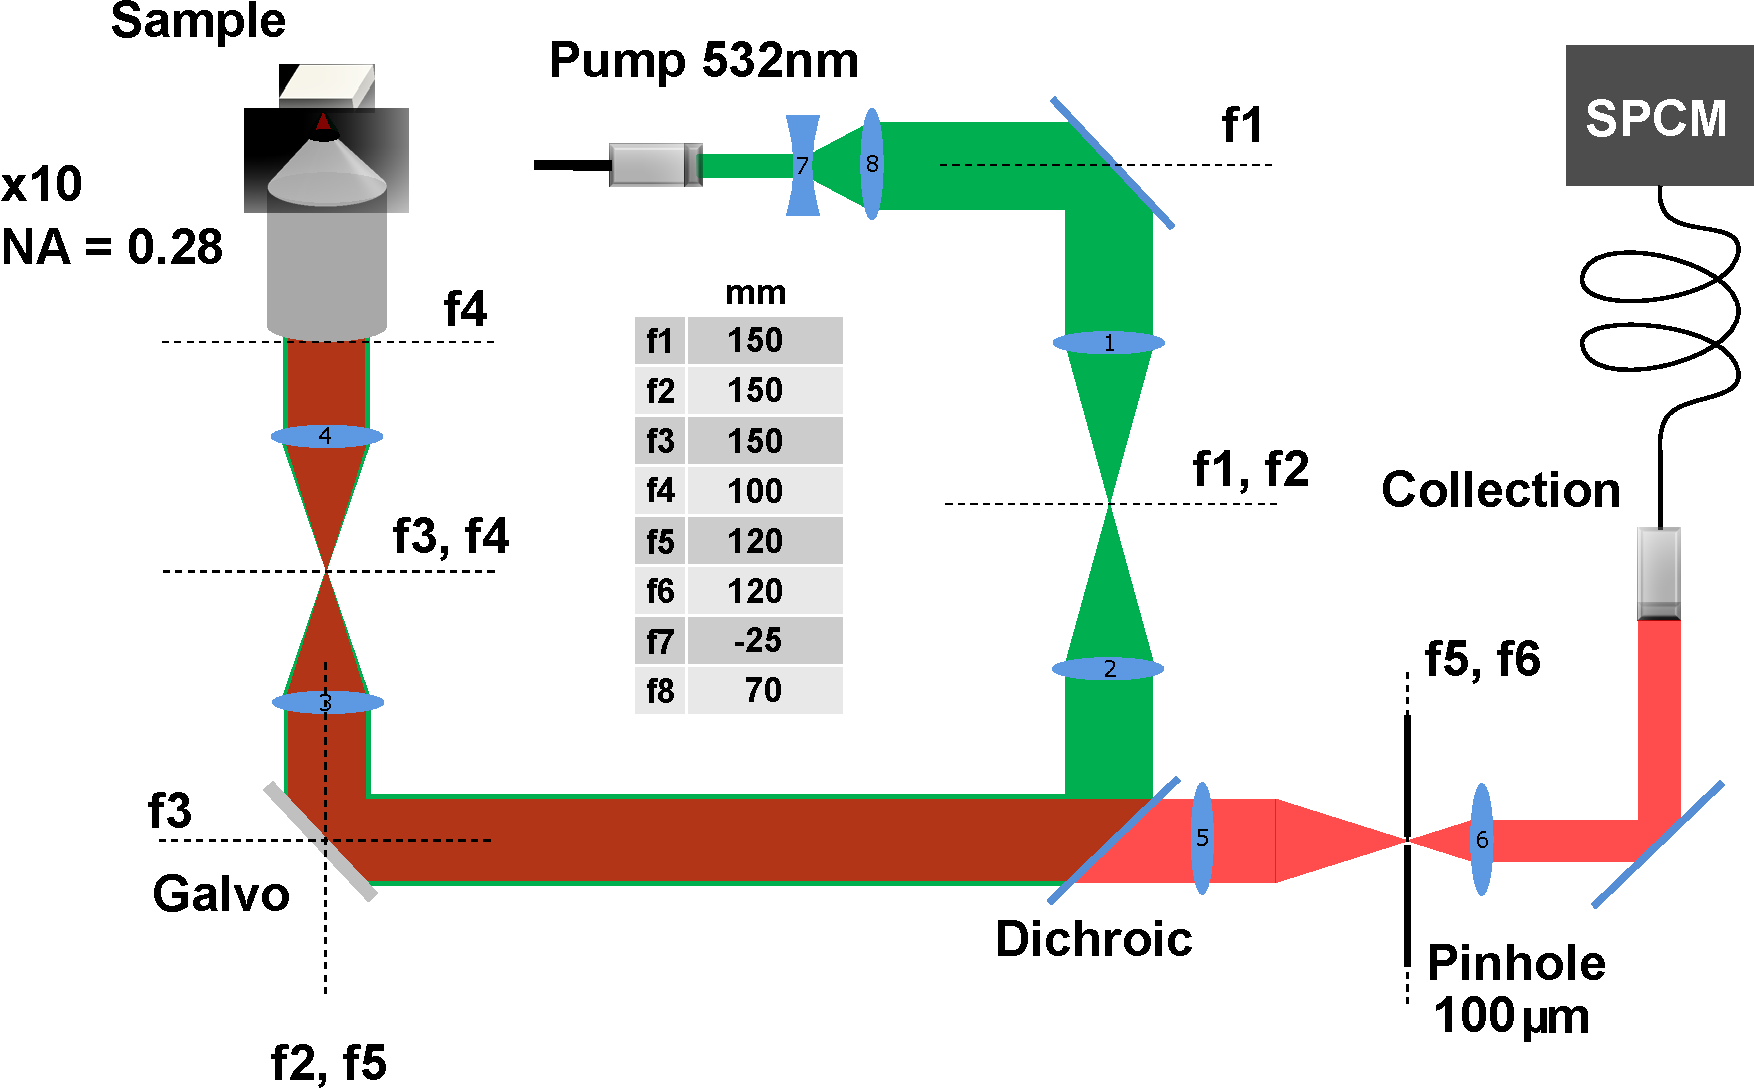
\includegraphics[scale = 0.7]{Confocal_Diagram_001.pdf}  
\caption{\textbf{Confocal Microscope} Custom built confocal microscope used to measure $B_1$ in LGR.}
\label{LGR_confocal_diagram}
\end{figure}
\end{landscape}

\subsection{Experimental setup} \label{setup}

To measure the field distribution within the LGR center loop a home-built scanning confocal microscope [Figure \ref{LGR_confocal_image}] was employed. The confocal microscope supplies the 532 nm pump beam to polarize the NVs and collects the resulting fluorescence using a dichroic beam splitter and a single photon counting module (SPCM). The three main sections of the experimental setup are the pump path, the collection path, and the sample path. The pump path [Figure \ref{LGR_confocal_diagram} (a)] includes all optics from the launch of the excitation beam to the dichroic. Optical pulsing is accomplished using an acousto-optic modulator (AOM) that is located before the fiber launch; Ie. the laser passes through an AOM and is then coupled into a single mode (SM) polarization maintaining fiber which is then launched as the pump beam. The SM fiber picks off the first order refracted beam of the AOM and rejects the rest so no iris needed. The pump path contains a fiber launch (FiberPort coupler PAF-X-11-B), a half wave plate to selectively excite and address NV orientations, a beam expander consisting of a positive and negative focal length lens, and a 1:1 telescope. The 1:1 telescope (ie. no magnification) serves to change the angle of the beam down the sample path without moving the excitation spot off the galvo mirrors. In order for this to happen, the distance between the center of the two galvo mirrors and the last lens of the telescope must be equal to the focal length of the lens. In this way the angle of the beam into the objective can be changed without needing to reposition the galvos---which is a function designed for convenience only. The beam expander changes the collimation of 532 nm into the objective and therefore changes where the green comes into focus along the optical axis of the objective. This effectively serves to overlap the green excitation and the red fluorescence. Overlapping the two beams serves to maximize collection through the pinhole on the collection arm since the pinhole is initially aligned using the back-reflected green pump laser.

\begin{figure}[t!]
\centering
\includegraphics[scale = 0.35]{DSC05087.jpg}  
\caption{\textbf{Image of Scanning Confocal Microscope} Custom built scanning confocal microscope used to measure the $B_1$ distribution in the LGR}
\label{LGR_confocal_image}
\end{figure}

The collection path (or arm) [Figure \ref{LGR_confocal_diagram} (b)] begins at the dichroic and ends at the collection end through a multimode fiber (65 $\upmu$m core) and into the SPCM. The path consists of the dichroic, a pinhole between two telescoping lenses, a multimode fiber, and an SPCM. The dichroic (Semrock Brightline FF552-Di02-25x36) filters the green pump beam from the sample fluorescence by reflecting wavelengths below 552nm and transmitting everything above. The first lens of the telescope focuses the beam down and passes it through a pinhole that spatially filters the image in X and Y to provide improved resolution. The pinhole was chosen to be 100 $\upmu$m to maximize collection while sacrificing some lateral resolution in the image. Generally the pinhole diameter ($p_d$) should be selected using the following equation:
\begin{equation}
p_d = \frac{1.22 \lambda}{NA} \cdot M_{objective} \cdot M_{telescope}. 
\end{equation}
The telescope in the sample path de-magnifies the beam by a factor $M_{telescope} = \frac{100}{150} = 0.67$ which is the ratio of the focal lengths of the lenses in the sample path. The objective used has a magnification of x10 which leads to a nominal pinhole size of 20 $\upmu$m. However, this limits the amount of fluorescence collected because the pinhole filters out-of-focal-plane light which constitutes a large part of the signal. Since measuring the $B_1$ field distribution in the LGR center cavity does not require high spatial resolution, a 100 $\upmu$m diameter pinhole was chosen such that each measurement wasn't fluorescence starved. The filtered beam then passes through a second lens which focuses it onto the core of a multimode fiber connected to the SPCM. The multimode fiber allows for some rejection of ambient light without too much loss of the fluorescence signal. To further minimize the collection of ambient light, the multimode fiber dock and SPCM are enclosed in a light tight box. 

The sample path [Figure \ref{LGR_confocal_diagram} (c)] also begins at the dichroic, but passes through the galvanometer and objective and ends at the sample within the LGR center loop. It consists of a galvanometer, a 4F lens system (telescope), an iris, an objective and a sample stage. The objective used (Mitutoyo 378-803-3, M Plan Apo 10x $\text{NA}=0.28$) has a long working distance of 34 mm. The long working distance was necessary to minimize perturbations of the $B_1$ field by the metal housing of the objective. Future NV wide-field imaging applications may require ceramic-tipped objectives. Finally, although this microscope has a galvanometer capable of scanning the beam over an area of $\sim$ 250 $\upmu$m x 250 $\upmu$m the beam was held steady and the resonator moved to ensure $B_0$ is consistent for all measurements across the central loop of the LGR.


\subsection{Measurement process} \label{measurement}

\begin{figure}[t!]
\centering
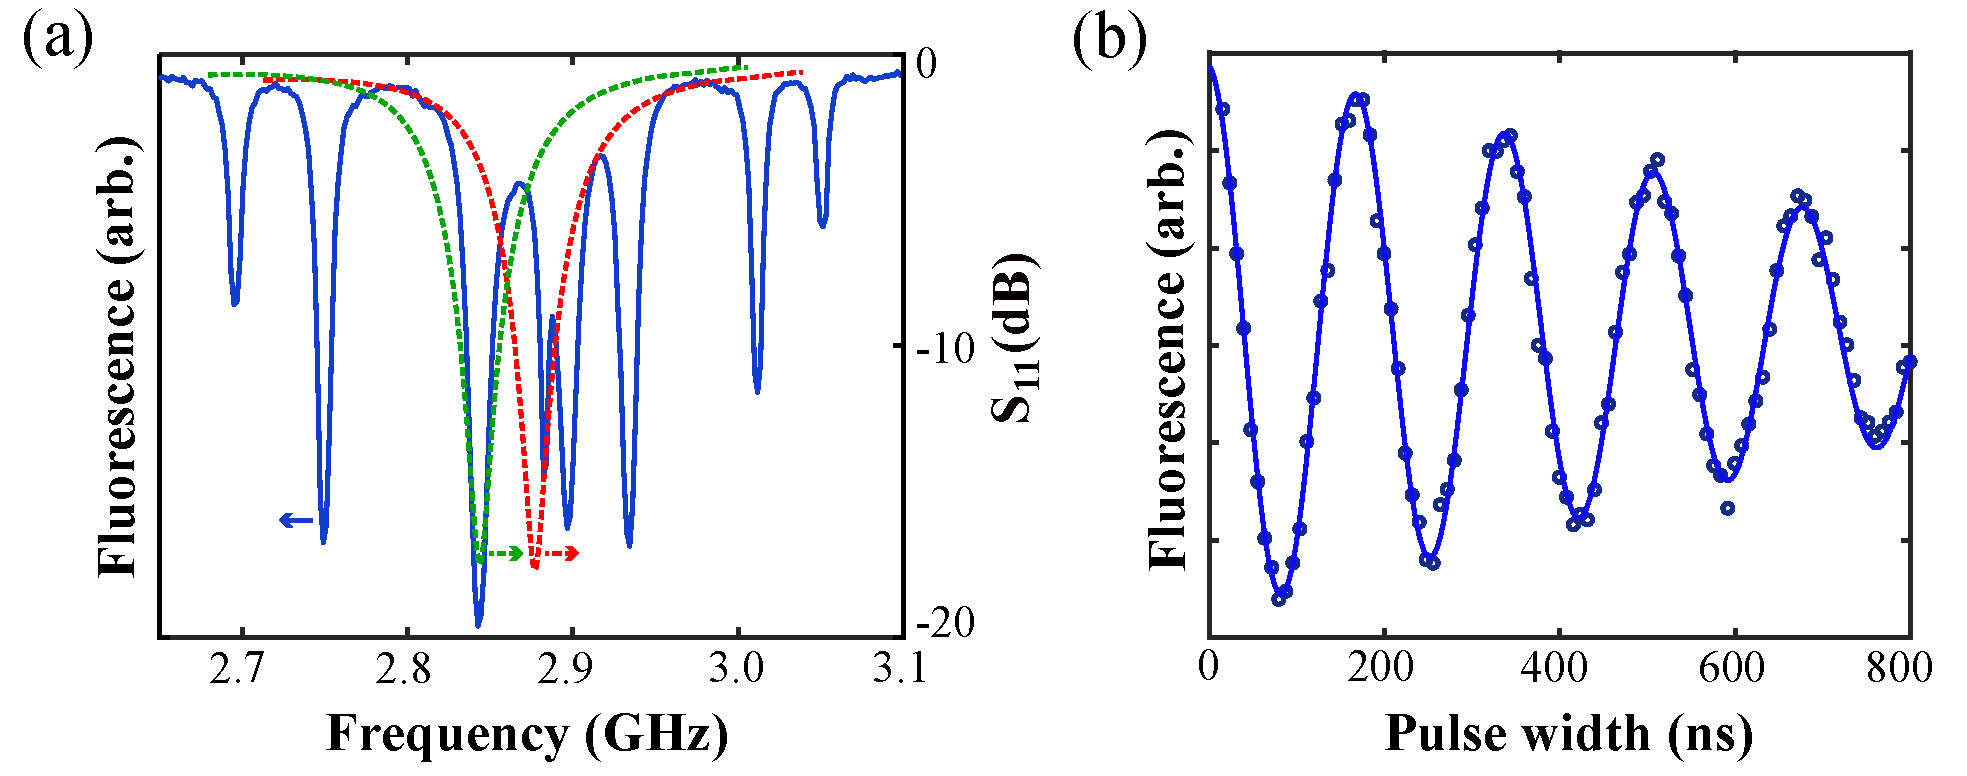
\includegraphics[scale = 0.45]{Figure_3.pdf}  
\caption{\textbf{LGR driving of an NV ensemble} \textbf{(a)} NV electron spin resonance spectrum (\textcolor{blue}{\textbf{---}}) under application of bias field $B_0$. The bias field allows individual addressing of all eight NV resonances, arising from the combination of the two allowed magnetic dipole transitions with the four possible NV orientations. The NV hyperfine structure is obscured by MW power broadening and the contrast variation between the NV resonances is attributed primarily to the $S_{11}$ line-shape. The $S_{11}$ parameter is shown before (\textcolor{red}{\textbf{-\,-\,-}}) and after (\textcolor{dolla-bill}{\textbf{-\,-\,-}}) shifting the LGR resonant frequency $f_0$ to the target NV resonance. Arrows indicate corresponding y axes. \textbf{(b)} Typical data depicting Rabi oscillations under MW excitation at the target NV resonance frequency indicated in (a). Data (\textcolor{navyblue}{$\mathbf{\circ}$}) is fit (\textcolor{blue}{\textbf{---}}) to an exponentially decaying sinusoid.}
\label{LGR_Rabi_meas}
\end{figure}

The strength and homogeneity of $B_1$ within the LGR central loop is evaluated employing standard NV techniques, as described in detail if references \cite{pham2013magnetic,childressthesis2011coherent,mazethesis2010quantum}. More specifically, a custom built scanning confocal microscope (as described in section \ref{setup}) measures the Rabi nutation frequency $\Omega_R$ of an ensemble of NV centers. A $\{$100$\}$-cut diamond plate containing $\sim 1 \times 10^{14}$ NV/cm$^3$ is mounted at the center of the LGR with the $<$100$>$ crystallographic axis collinear with the LGR axis. A rare earth magnet creates a static magnetic bias field $B_0$, which shifts the energies of the $m_s=\pm1$ ground-state Zeeman sublevels. The energy shifts are given to first order by~\cite{taylor2008high}
\begin{equation}
\Delta E \approx \text{g}_{\text{s}} \upmu_\text{B} m_s \vec{B}_0\cdot \hat{n}_i,
\end{equation}
where $\hat{n}_i$ denotes a unit vector oriented along one of the four diamond crystallographic axes. By judicious choice of $\vec{B}_0$, all eight energy levels and associated $m_s\!=\!0\! \leftrightarrow \!m_s\! =\!\pm1$ magnetic dipole transitions can be isolated as shown in Fig. \ref{LGR_Rabi_meas}(a). The resonator is tuned to excite a single NV transition, yielding Rabi oscillations [Fig. \ref{LGR_Rabi_meas}(b)]. The data is fit to an exponentially decaying sinusoid in order to extract the Rabi frequency $\Omega_R$, from which the magnitude of $B_1$ can be calculated as
\begin{equation}\label{B1fromRabi}
B_1 = \sqrt{3}\frac{\hbar \Omega_R}{\text{g}_{\text{s}} \upmu_{B}}.
\end{equation} 
In this geometry, the $B_1$ field is oriented along the [100] crystallographic axis of the diamond, degenerately offset from all four NV axis orientations by half the tetrahedral bond angle $\theta_{\text{tet}}/2 = \text{ArcCos}\frac{1}{\sqrt{3}} \approx 54^\circ$. NV Rabi oscillations are driven by the $B_1$ field component transverse to the NV symmetry axis, reducing the Rabi frequency by $\sqrt{2/3}$ \cite{sasaki2016broadband}. Accounting for the rotating wave approximation introduces another factor of $1/\sqrt{2}$ resulting in the conversion factor $\sqrt{3}$ in equation \ref{B1fromRabi}. To ensure $\vec{B}_0$ is consistent for all measurements across the LGR central loop, the confocal excitation volume is held fixed with respect to the $B_0$-generating permanent magnet, and the diamond and LGR composite device are translated together. The process is then repeated at a locus of points within the LGR center loop (discussed below in section \ref{LGRfield}).

%A static magnetic field ($B_0$) is applied to split the NV resonances and the sapphire shims (tuning process described in section \ref{tuning} are adjusted to tune the resonator to a single NV resonance as shown in Figure \ref{LGR_Rabi_meas} (a). A long working distance objective collects the NV fluorescence while its 34 mm working distance mitigates the effect of the metal objective housing on $B_1$. To measure $\Omega_R$ the NVs within the confocal volume are consecutively polarized, driven, and read out while sweeping the pulse length of the MW driving field. Using a gated single photon counting module, the fluorescence is collected and plotted against the MW pulse length

% Talk about experiment taking Rabi data, ie. Rabi pulse sequence, moving resonator, checking ESR, choosing ESR etc.

%\subsection{$B_1$ from Rabi} \label{calcRabi}
%
%calculating $B_1$ from Rabi frequency using rotating wave approx. etc, essentially where sqrt(3) comes from.


\begin{figure}[t!]
\centering
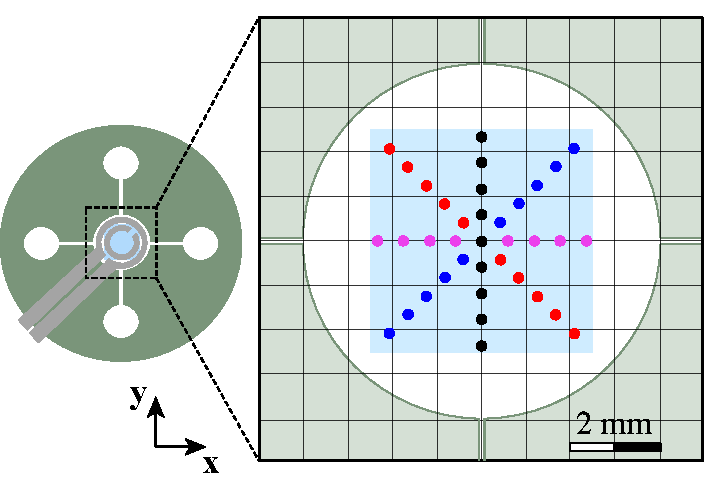
\includegraphics[scale = 1]{Locus_Points.pdf}  
\caption{\textbf{Locus of Measurement Points}  An NV-containing 4.5 mm $\times$ 4.5 mm diamond plate is placed in the LGR central loop, and the  Rabi frequency is measured where indicated (\textcolor{deepmagenta}{\textbullet},\textcolor{black}{\textbullet},\textcolor{red}{\textbullet},\textcolor{blue}{\textbullet}) to characterize $B_1$.}
\label{LGR_Locus}
\end{figure}


\section{LGR field distribution} \label{LGRfield}

The measurement described above is applied at a locus of points in the center of the LGR [Figure \ref{LGR_Locus}]. Since the field distribution is radially symmetric the rest of the field values can be determined from the provided measurements. Application of incident MW power $P \approx 42$ dBm yields an axially oriented $B_1$ at the center of the LGR with magnitude 4.7 G. The corresponding Rabi frequency $\Omega_R = 2\pi \times 7.7$ MHz for NV centers oriented at half the tetrahedral bond angle relative to the LGR axis. Qualitatively, as shown in Figure \ref{LGR_Field_Image} $B_1$ (calculated using equation \ref{B1fromRabi})displays a minimum at the LGR center, increases in magnitude with increasing radial displacement from the center, and is approximately radially symmetric. The best homogeneity is therefore expected at the LGR center. Using equations \ref{sigma_rms} and \ref{sigma_pp} we calculate that, over a 32 mm\textsuperscript{2} circular area axially centered in the LGR
central loop, we observe $\sigma_{rms} = 3.2\%$ and $\sigma_{pp} = 10.5\%$, as shown in Figure \ref{LGR_Field_Image}. Over a smaller 11 mm\textsuperscript{2} circular area, a $\sigma_{rms} = 1.6\%$ and $\sigma_{pp} = 3\%$ is observed. Additionally, as a three-dimensional cavity resonator, the LGR provides better axial field uniformity than planar-only geometries \cite{floch2016towards,kapitanova2017dielectric,angerer2016collective}. For example, for a 3.14 mm\textsuperscript{3} cylindrical volume (1 mm radius disk with 1 mm thickness), simulations yield $\sigma_{\text{rms}}=0.8\%$, $\sigma_{\text{pp}}=3.7\%$ and an average $B_1$ of 4.8 G (see section \ref{simField}).


\begin{figure}[t!]
\centering
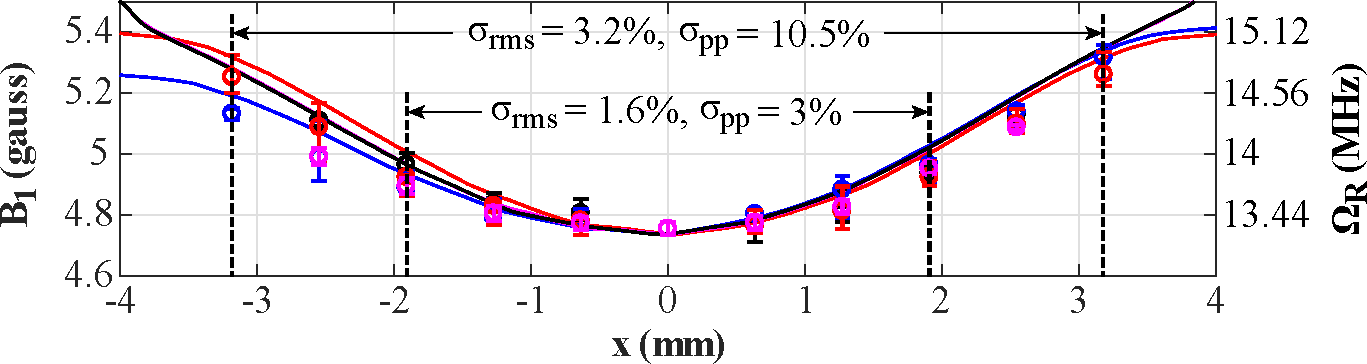
\includegraphics[scale = 0.7]{B1Field.pdf}  
\caption{\textbf{$\boldsymbol{B_1}$ field uniformity of LGR composite device.} $B_1$ field measurements (\textcolor{deepmagenta}{$\circ$},\textcolor{black}{$\circ$},\textcolor{red}{$\circ$},\textcolor{blue}{$\circ$}) at the points depicted in \ref{LGR_Locus} and simulations (\textcolor{deepmagenta}{\textbf{--}},\textcolor{black}{\textbf{--}},\textcolor{red}{\textbf{--}},\textcolor{blue}{\textbf{--}}) along each locus of points are in good agreement. Error bars indicate 1-sigma uncertainty for the $B_1$ measurement. Dashed lines indicate the radial boundaries of the 32 mm$^2$ and 11 mm$^2$ areas over which $B_1$ field uniformity is evaluated. The measured $B_1$ uniformity is given for each area.}
\label{LGR_Field_Image}
\end{figure}



